\scanpage{46}
$A$ variété abélienne en. car $p$. On a, pour la partie de $\pi_1(A)$ première à $p$
\[
\pi_1^{\neq p}(A)\simeq\varprojlim_{\substack{n\\\text{arith}\\(n,p)=1}}\deleted{\unsure{n}}A^{(n)}
\]
où $\deleted{\unsure{n}}A^{(n)}$ est le noyau de $A\xrightarrow{n}A$, et où $A^{(mn)}\mathbin{-}A^{(n)}$ est la multiplication par $m$.
\[
\vcenter{\hbox{\begingroup
\setbox0=\hbox{$\displaystyle \pi_1^\ell(A)\simeq\varprojlim_{\deleted{\unsure{\ell}}k} A^{(\ell^k)}\simeq T_\ell(A)=\operatorname{Hom}(\underline{\mathbb Q}_\ell/\mathbb Z_\ell,A)$}
\dimen0=\wd0 \advance\dimen0 by 18pt
\dimen2=\ht0 \advance\dimen2 by \dp0 \advance\dimen2 by 16pt
\rlap{\raisebox{\dimexpr-\dp0-8pt\relax}{%
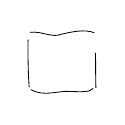
\begin{tikzpicture}[x={\dimexpr\dimen0/1256\relax},y={\dimexpr-\dimen2/177\relax},line width=.3pt]
\path[use as bounding box] (0,0) rectangle (1256,177);
\draw (41,12) .. controls (250,8) and (450,27) .. (610,17) .. controls (800,11) and (1030,3) .. (1217,13);
\draw (8,31) .. controls (2,63) and (8,116) .. (27,153);
\draw (58,159) .. controls (310,179) and (545,161) .. (785,164) .. controls (975,165) and (1155,166) .. (1192,156);
\draw (1235,65) .. controls (1243,78) and (1236,116) .. (1245,155);
\end{tikzpicture}}}%
\kern9pt\box0\kern9pt\endgroup}}
\]
\margin{module de Tate}
$\ell$ étant un nb premier $\neq p$. Ce résultat provient du fait qu'un \uline{revêtement non ramifié d'une variété abélienne est une variété abélienne}

D'après Kummer, on a d'autre part
\[
\deleted{\text{\unsure{Dual|Donc}}}\operatorname{Hom}(\pi_1^\ell(A),U_\ell)\simeq
\text{sous-gpe de }\unsure{\mathfrak P|\mathfrak D}(A)=H^1(A,\underline O_{\unsure{A|\Lambda}}^{\unsure{*}})
\]
des \unsure{élém\textsuperscript{ts}|élts} d'ordre une puissance de $\ell$.

Si on admet que \uline{$A$ n'a pas de torsion}, on obtient donc
\[
\operatorname{Hom}(\pi_1^\ell(A),U_\ell)\simeq A^{*(\ell^\infty)},\qquad\text{i.e.}
\]
\[\boxed{T_\ell(A)\times T_\ell(A^*)\longrightarrow T_\ell(U_\ell)}\]
accouplement à valeurs dans le $\mathbb Z_\ell$-module libre de rang 1 $T_\ell U_\ell)$, et accouplement qui est une dualité.
\[
T_\ell(A)/\ell^kT_\ell(A)\times T_\ell(A^*)/\ell^{\unsure{k|n}}T_\ell(A')\longrightarrow
T_\ell(U_\ell)/\ell^kT_\ell U_\ell)
\]
\[A^{(\ell^{\unsure{k|n}}]}\times A^{*(\ell^k)}\longrightarrow U^{(\ell^{\unsure{k|n}})}\]
\margin{45}
